\section{Задание 1. Интегральная сумма}
\subsection{Интегральная сумма}
\subsection*{Задание}
Исследуйте интегральную сумму функции $ \frac{1}{1 + x^2} $,заданной на отрезке $ \left[-1;\sqrt{3}\right]$
\subsection*{Интегральная сумма функции на заданном отрезке в виде ступенчатой фигуры}
\begin{center}
	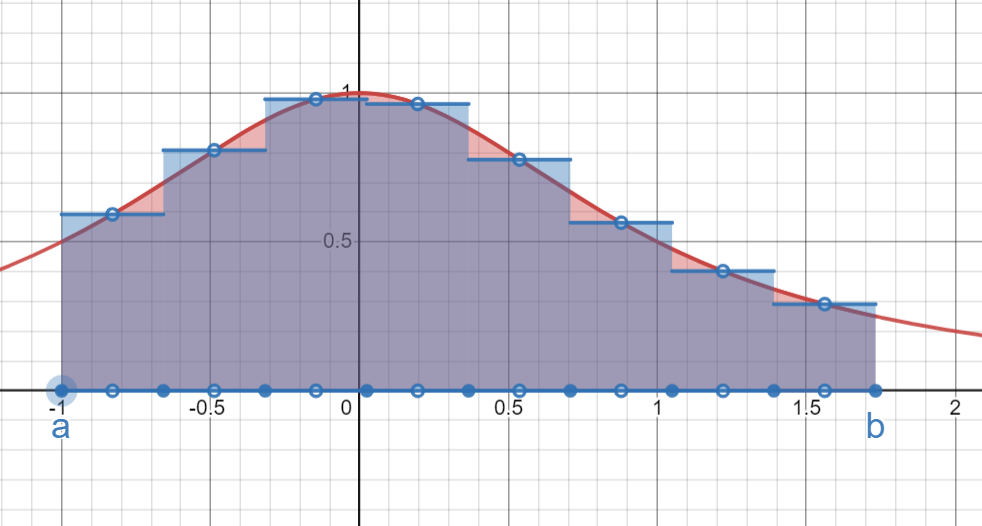
\includegraphics[width=0.4\linewidth]{task1_img1}\\
	\url{https://www.desmos.com/calculator/w21pp71fpr}
\end{center}
\subsection*{Исследование ступенчатой фигуры}
Рассмотрим разбиение на 3, 8 и 50 ступеней:
\begin{figure}[H]
	\centering
	\begin{subfigure}{0.3\textwidth}
		\centering
		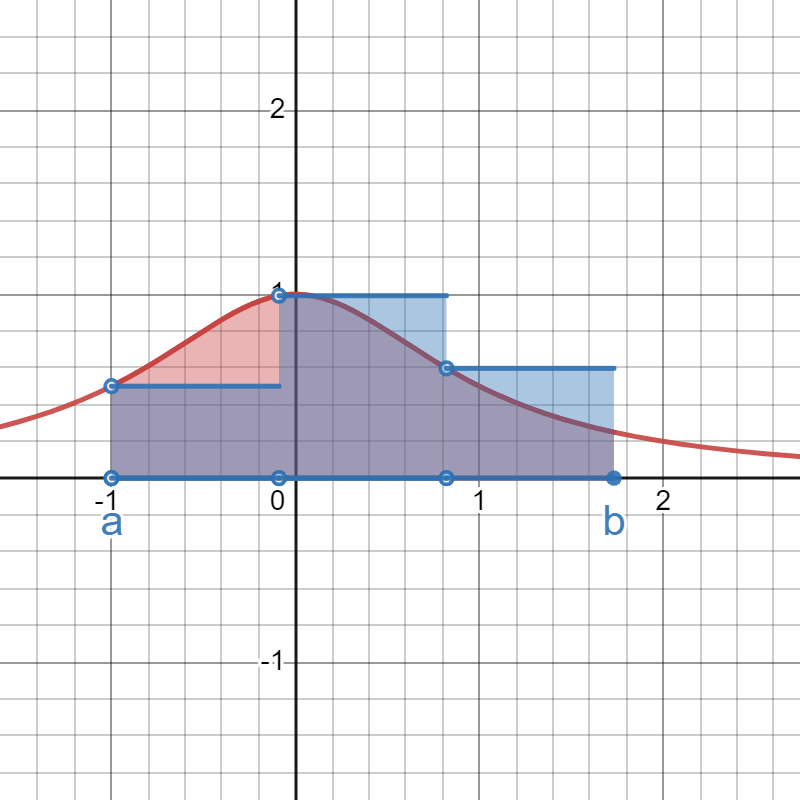
\includegraphics[width=.8\linewidth]{task1_n3_left}\quad
		\caption*{Крайнее левое положение точек}
	\end{subfigure}
	\begin{subfigure}{0.3\textwidth}
		\centering
		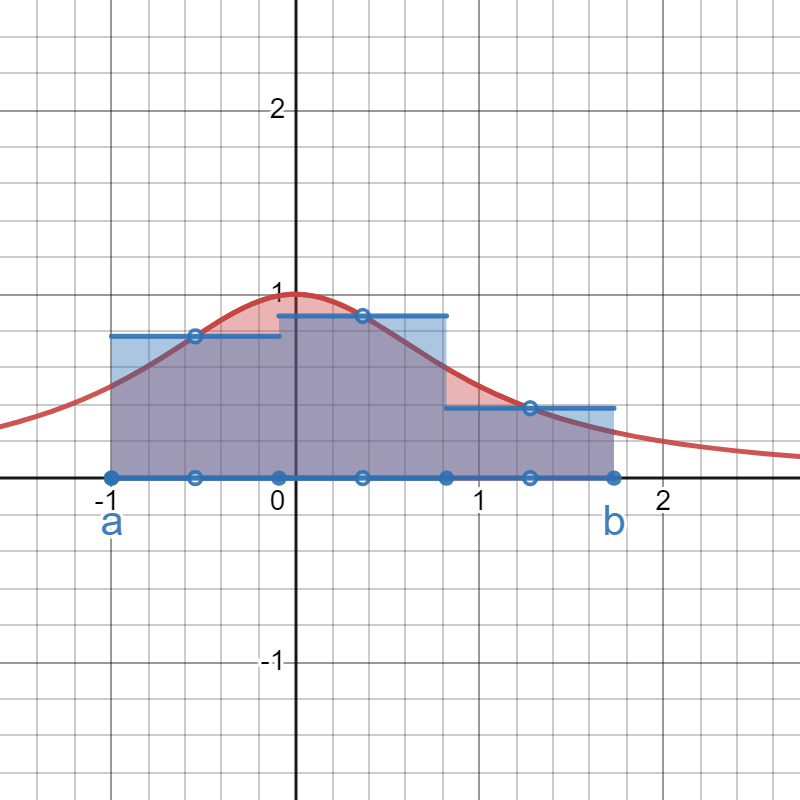
\includegraphics[width=.8\linewidth]{task1_n3_middle}\quad
		\caption*{Промежуточное положение точек}
	\end{subfigure}
	\begin{subfigure}{0.3\textwidth}
		\centering
		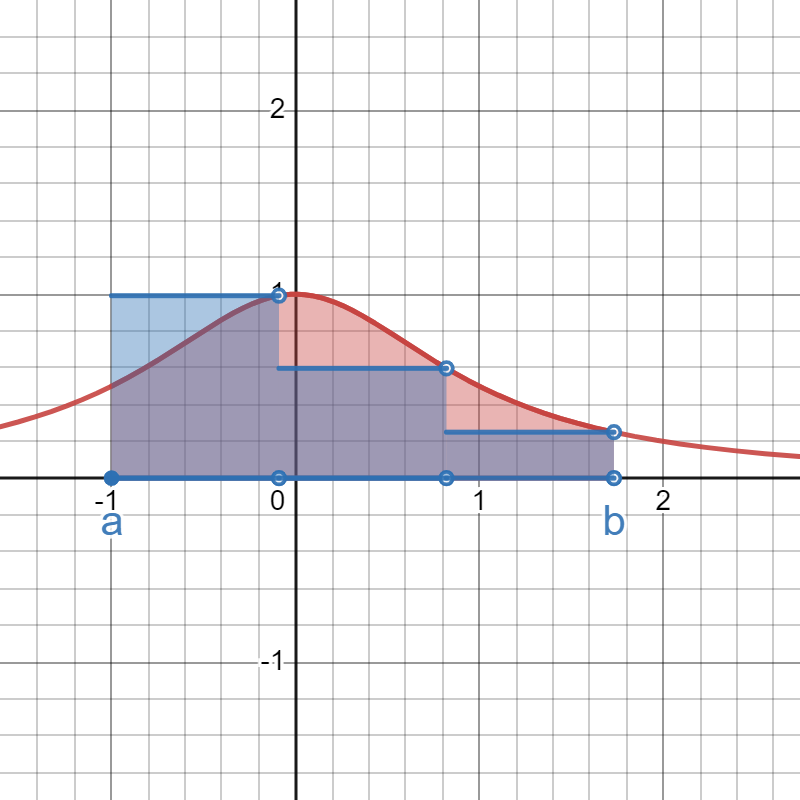
\includegraphics[width=.8\linewidth]{task1_n3_right}\quad
		\caption*{Крайнее правое положение точек}
	\end{subfigure}
	\caption{Разбиение на 3 ступени}
\end{figure}

\begin{figure}[H]
	\centering
	\begin{subfigure}{0.3\textwidth}
		\centering
		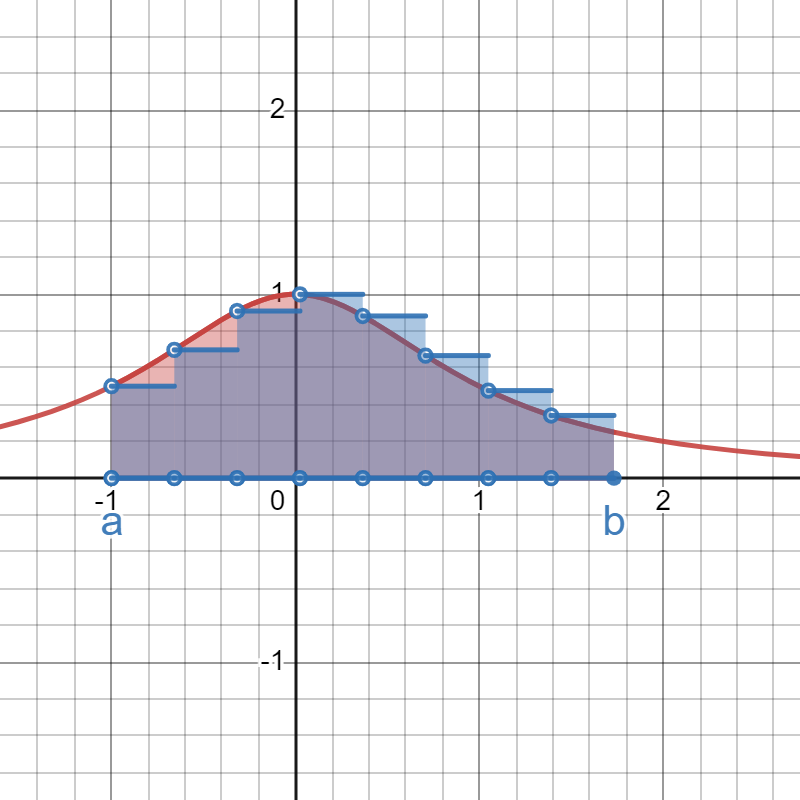
\includegraphics[width=.8\linewidth]{task1_n8_left}\quad
		\caption*{Крайнее левое положение точек}
	\end{subfigure}
	\begin{subfigure}{0.3\textwidth}
		\centering
		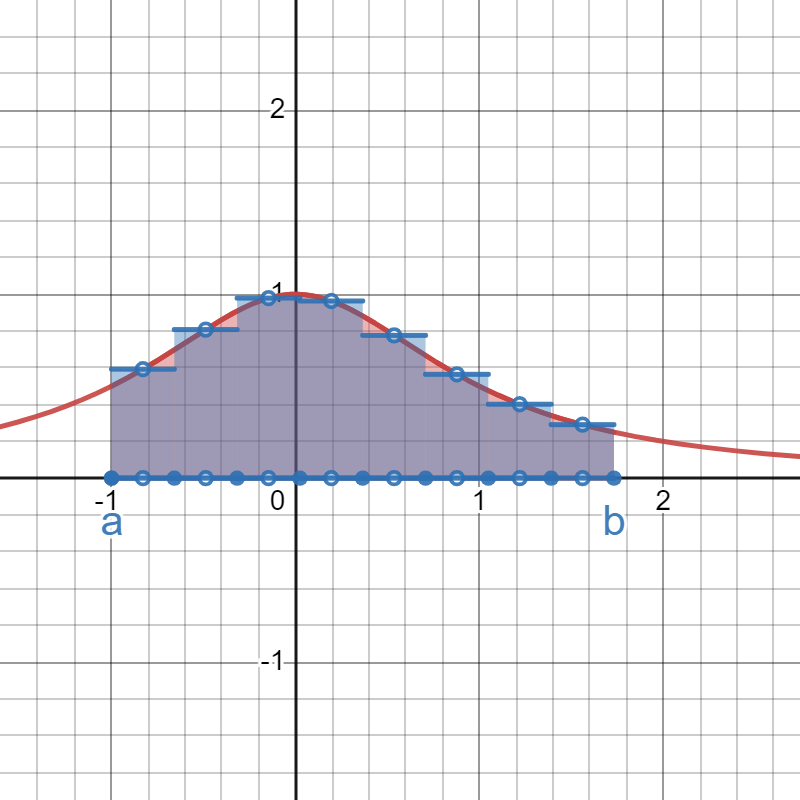
\includegraphics[width=.8\linewidth]{task1_n8_middle}\quad
		\caption*{Промежуточное положение точек}
	\end{subfigure}
	\begin{subfigure}{0.3\textwidth}
		\centering
		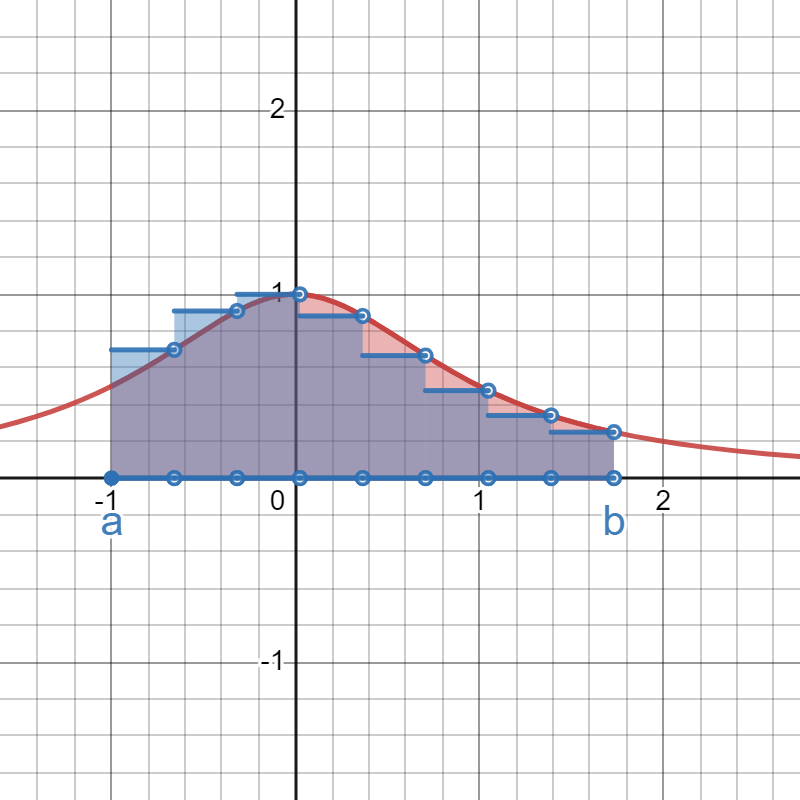
\includegraphics[width=.8\linewidth]{task1_n8_right}\quad
		\caption*{Крайнее правое положение точек}
	\end{subfigure}
	\caption{Разбиение на 8 ступеней}
\end{figure}

\begin{figure}[H]
	\centering
	\begin{subfigure}{0.3\textwidth}
		\centering
		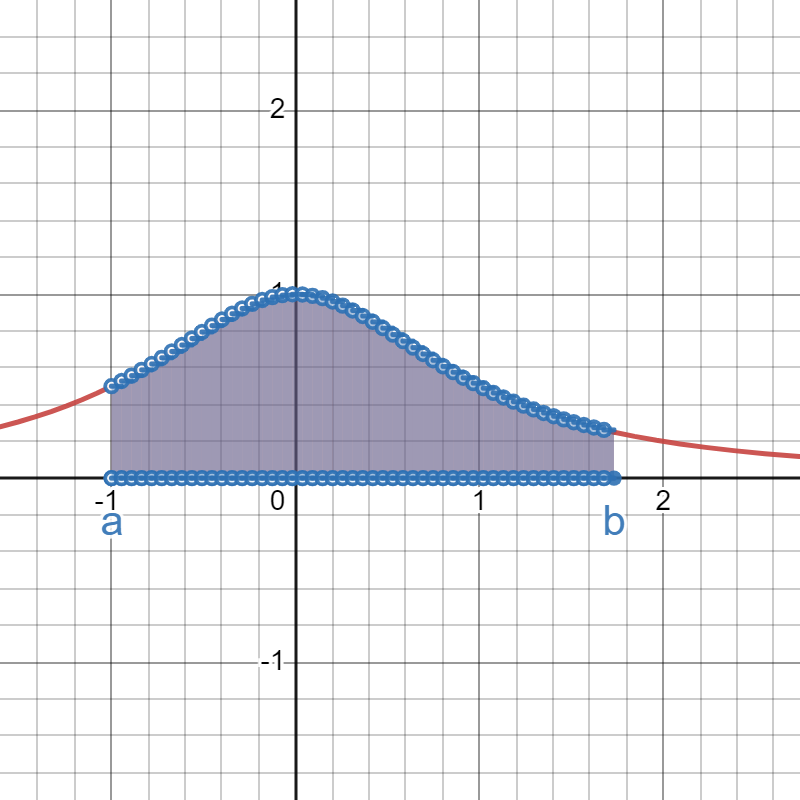
\includegraphics[width=.8\linewidth]{task1_n50_left}\quad
		\caption*{Крайнее левое положение точек}
	\end{subfigure}
	\begin{subfigure}{0.3\textwidth}
		\centering
		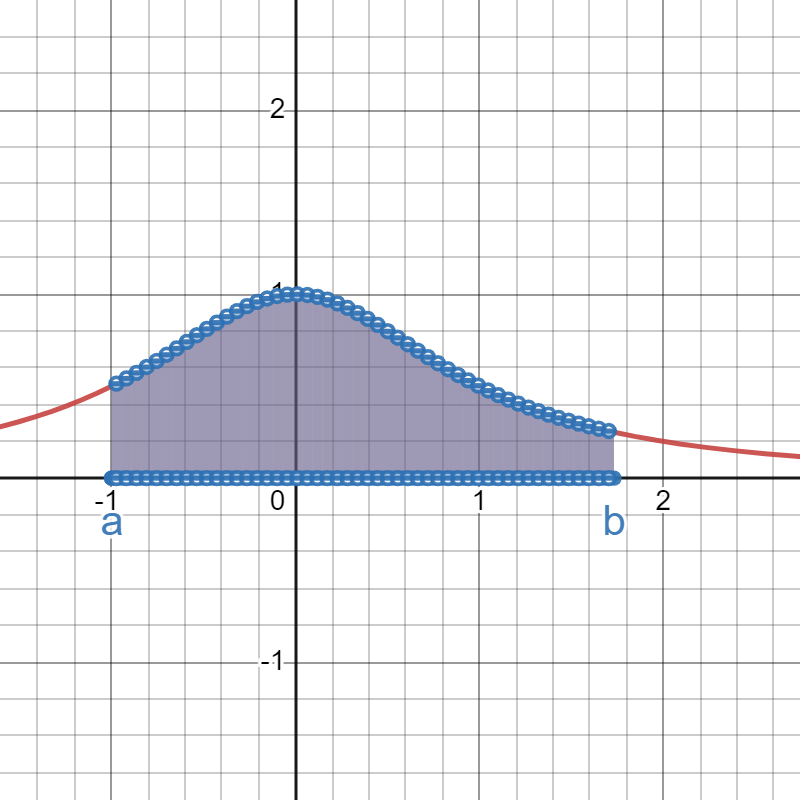
\includegraphics[width=.8\linewidth]{task1_n50_middle}\quad
		\caption*{Промежуточное положение точек}
	\end{subfigure}
	\begin{subfigure}{0.3\textwidth}
		\centering
		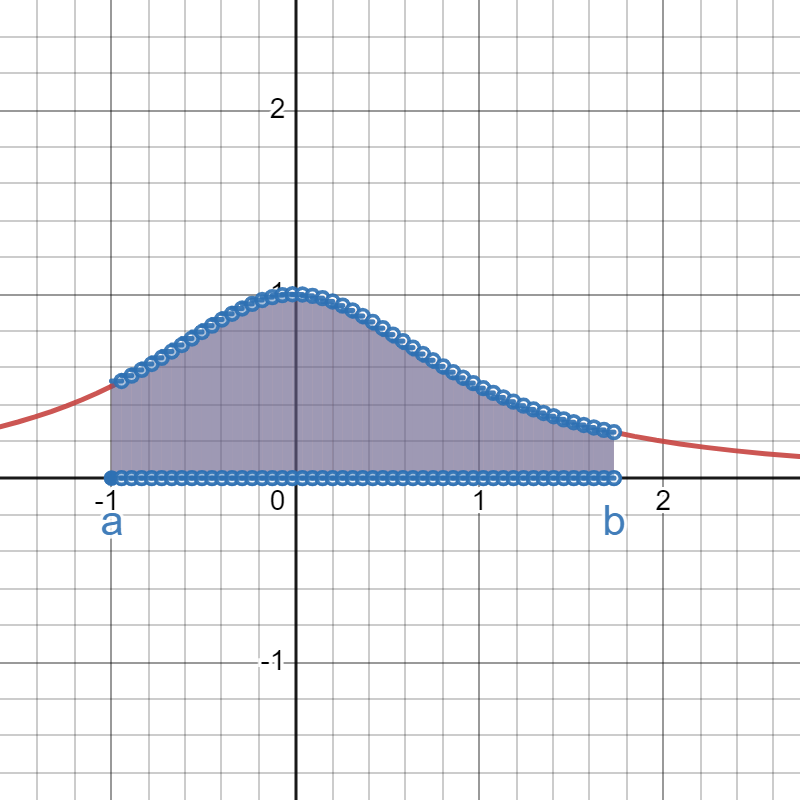
\includegraphics[width=.8\linewidth]{task1_n50_right}\quad
		\caption*{Крайнее правое положение точек}
	\end{subfigure}
	\caption{Разбиение на 50 ступеней}
\end{figure}
\subsection*{Заключение}
В процессе выполнения первого задания были построены ступенчатые фигуры по графику и исследованы зависимости точности вычислений от количества и положения точек. Точность вычисления прямо пропорциональна количеству точек, которые мы берем на отрезке. Так же следует брать точки приближенные к середине дробления, потому что в иных случаях результат получится менее точным.

